\chapter{Аналитический раздел}
\label{cha:analysis}

Облака - очень сложная и выразительная часть неба. Именно облака могут создать впечатление
о надвигающихся погодных условиях.
Для создания реалистичного неба облака должны визуализироваться в реальном времени.
Есть множество алгоритмов для достижения этой цели.

\section{Методы создания облаков}

Существует три основных метода визуализации облаков. Классический метод подразумевает использование единой панорамной текстуры,
которую необходимо наложить на небесную сферу \cite{Gue14}. Чтобы создать движение в небе, используется техника визуального
потока, при котором панорамная текстура вращается, создавая иллюзию движения облаков в определенном направлении, например,
ветра (рисунок \ref{img:cloud_sphere}). Данный метод является эффективным, однако не позволяет изменять форму облаков, погоду или освещение
(рисунок \ref{img:result_sphere}).

\begin{figure}[H]
    \centering
    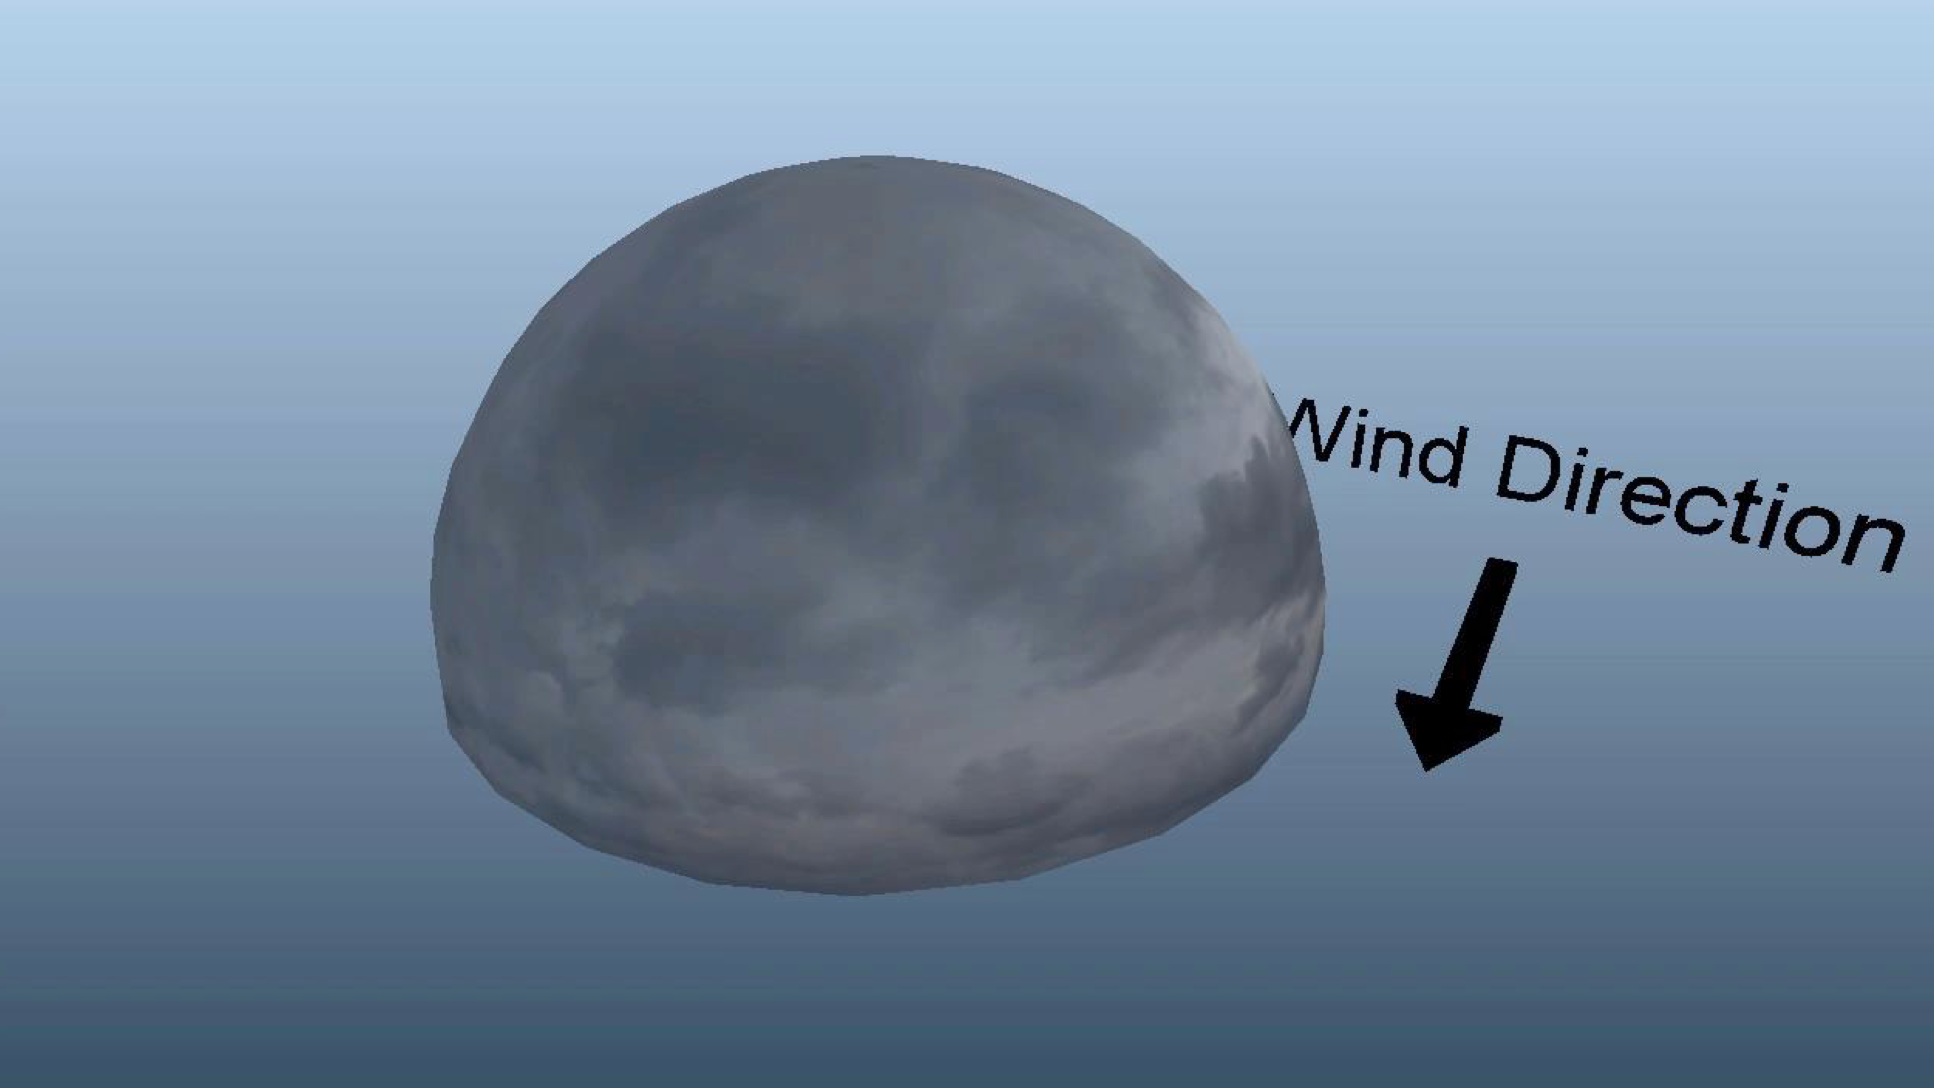
\includegraphics[scale=0.4]{img/cloud_sphere.png}
    \caption{Классический метод визуализации облаков}
    \label{img:cloud_sphere}
\end{figure}

\begin{figure}[H]
    \centering
    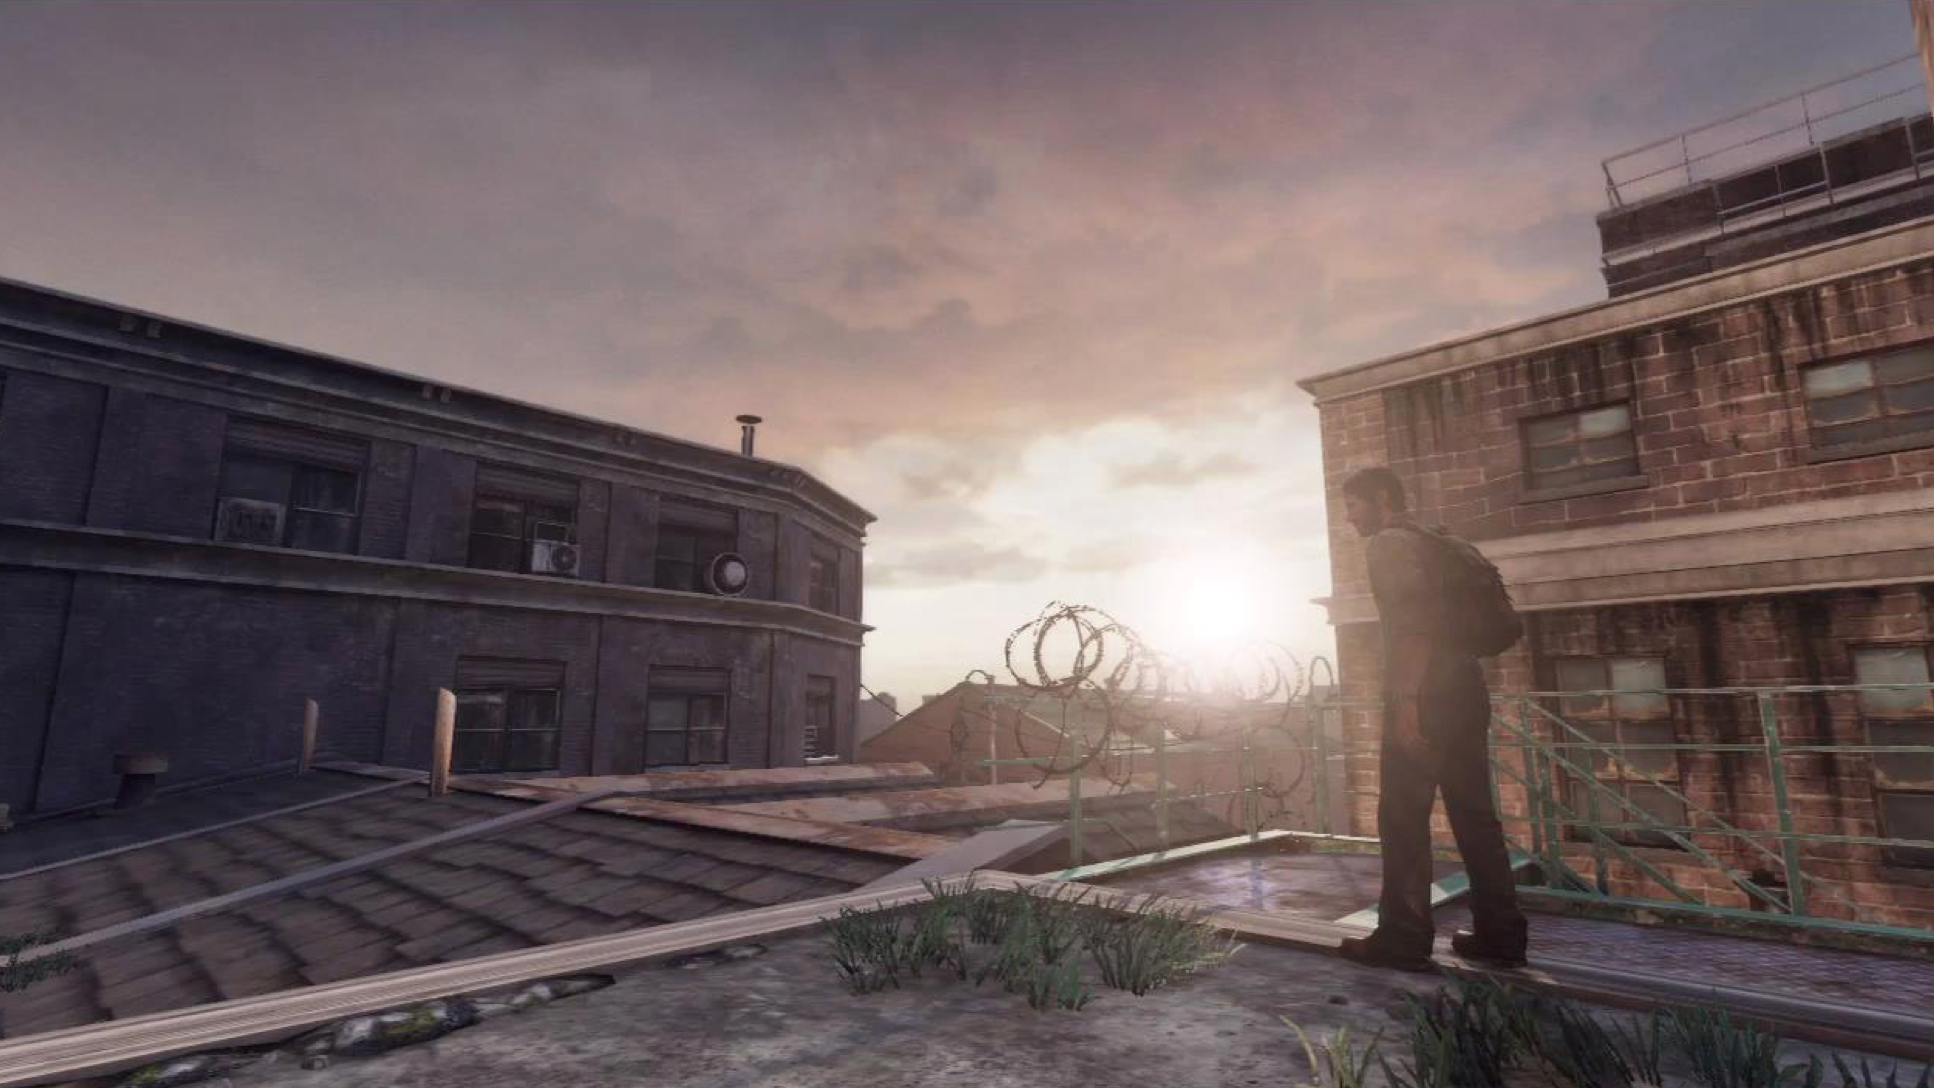
\includegraphics[scale=0.4]{img/result_cloud_sphere.png}
    \caption{Результат классического метода визуализации облаков}
    \label{img:result_sphere}
\end{figure}

При необходимости учета динамического освещения солнца можно генерировать облака при помощи частиц \cite{hpg.20141101}.
Такой метод требует больших затрат по времени, но облака получаются объемными и к ним можно приближать камеру.

\begin{figure}[H]
    \centering
    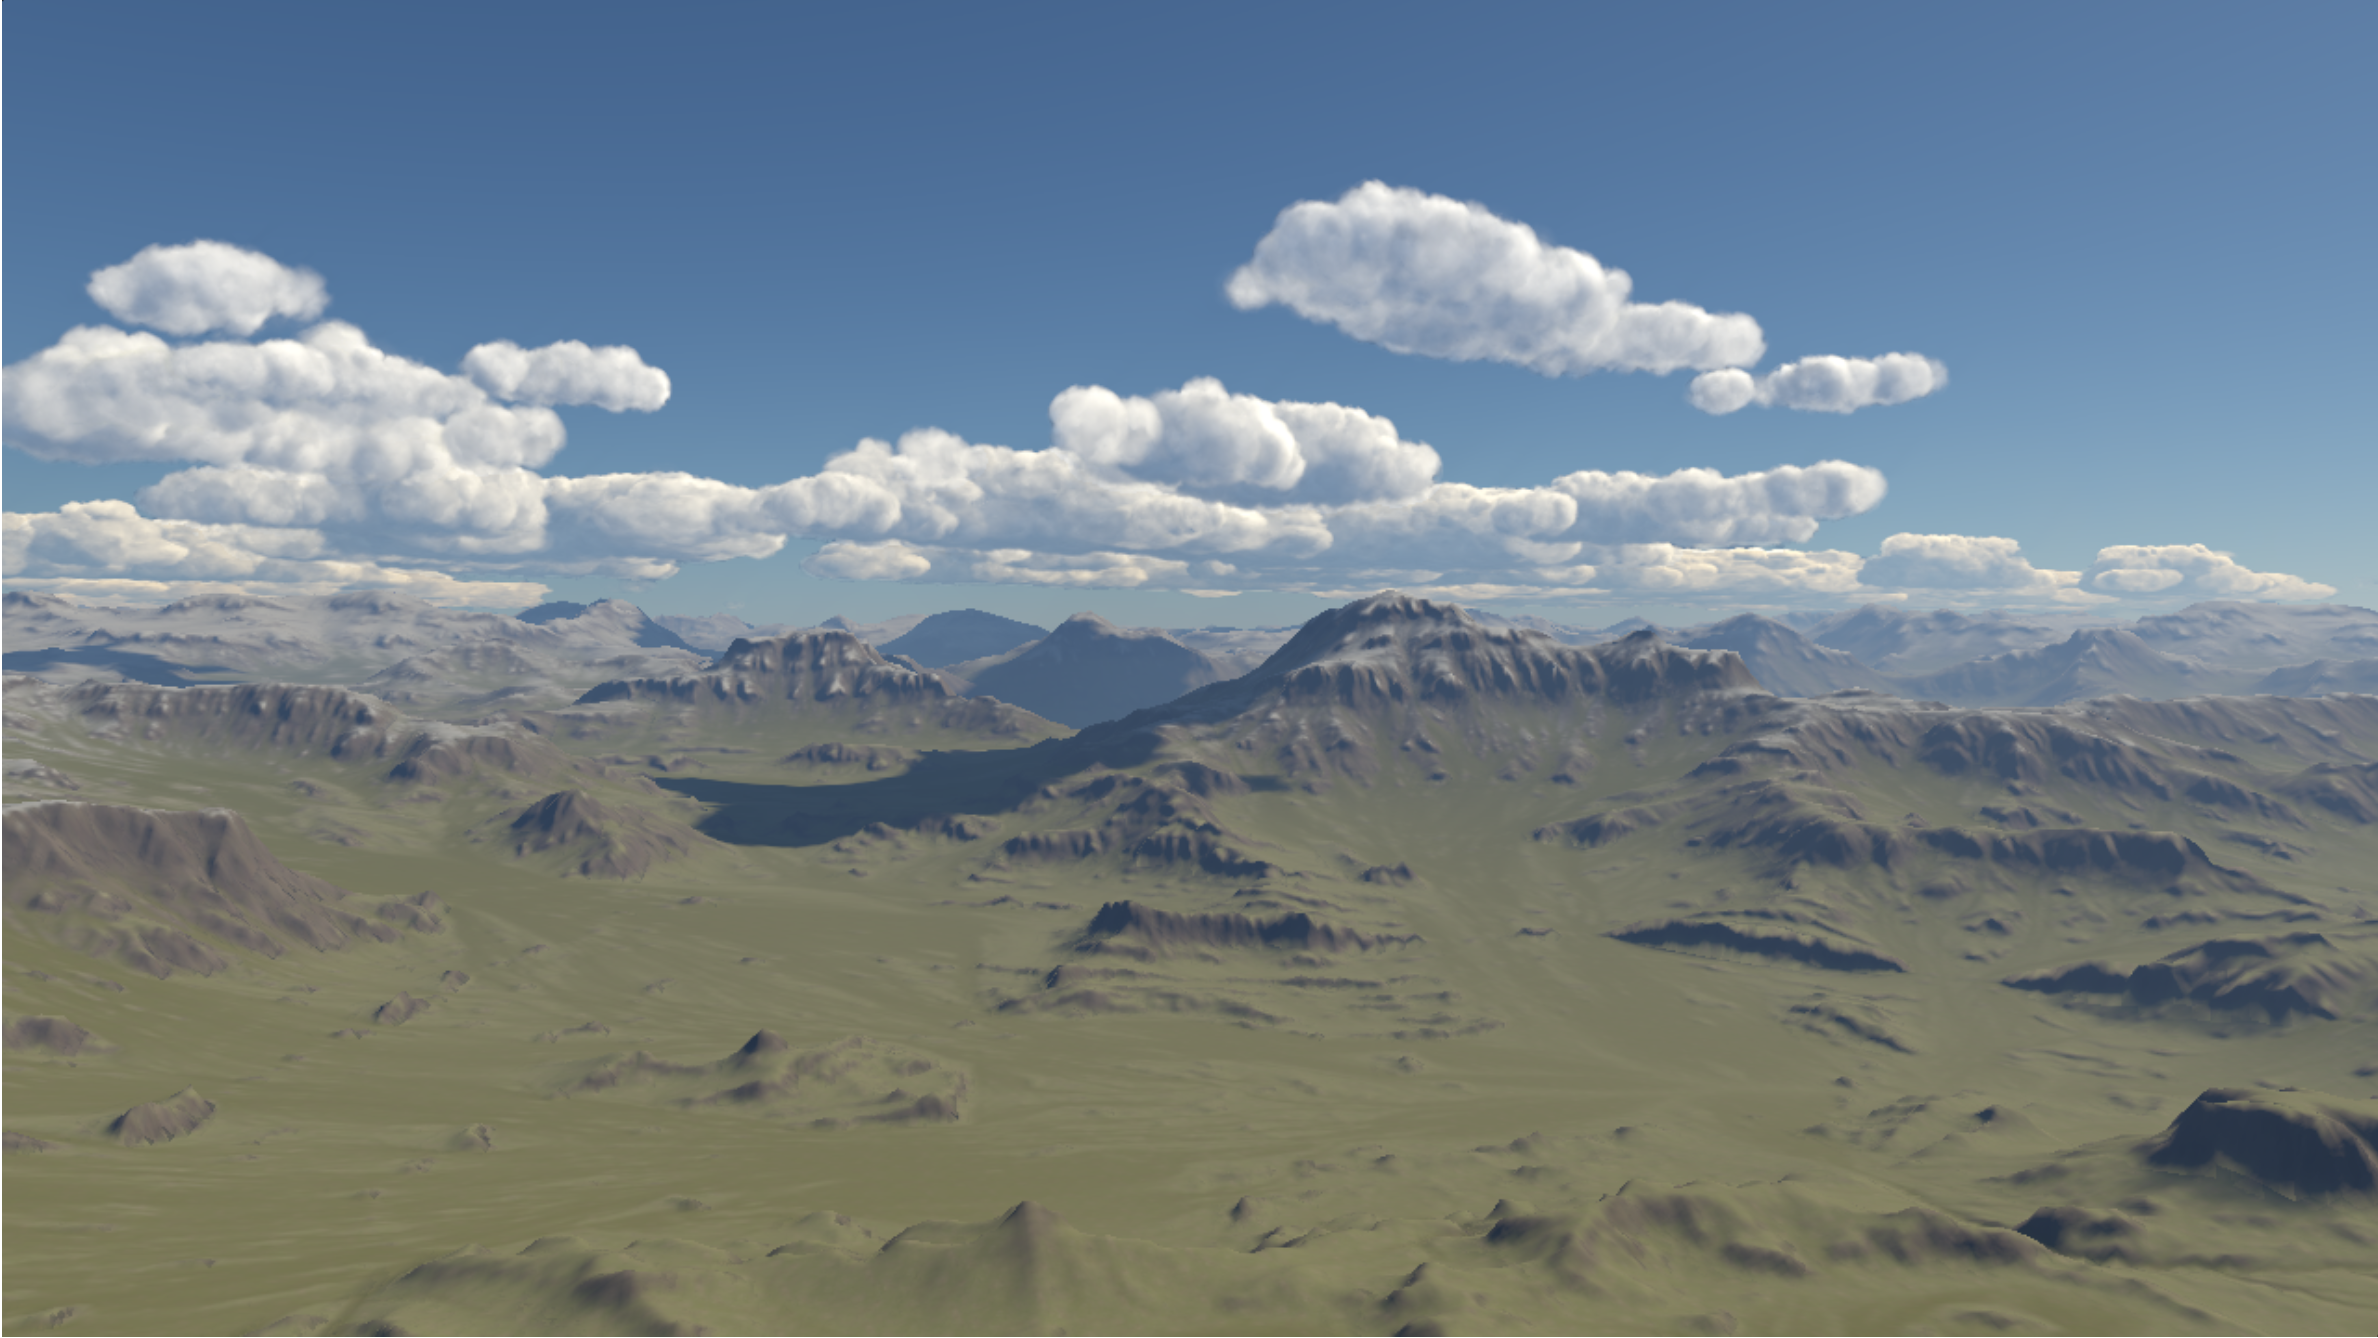
\includegraphics[scale=0.4]{img/ysov.png}
    \caption{Результат алгоритма частиц}
    \label{img:ysov}
\end{figure}

Третий метод называется алгоритм трассировки лучей, являющий самым трудоемким из всех алгоритмов
визуализации облаков. Данный алгоритм позволяет визуализировать динамически освещенные
облака \cite{Sch16}. С помощью нескольких параметров этот метод позволяет строить сложные облачные
формы с высокой детализацией как видно на рисунке \ref{img:raymach}.

\begin{figure}[H]
    \centering
    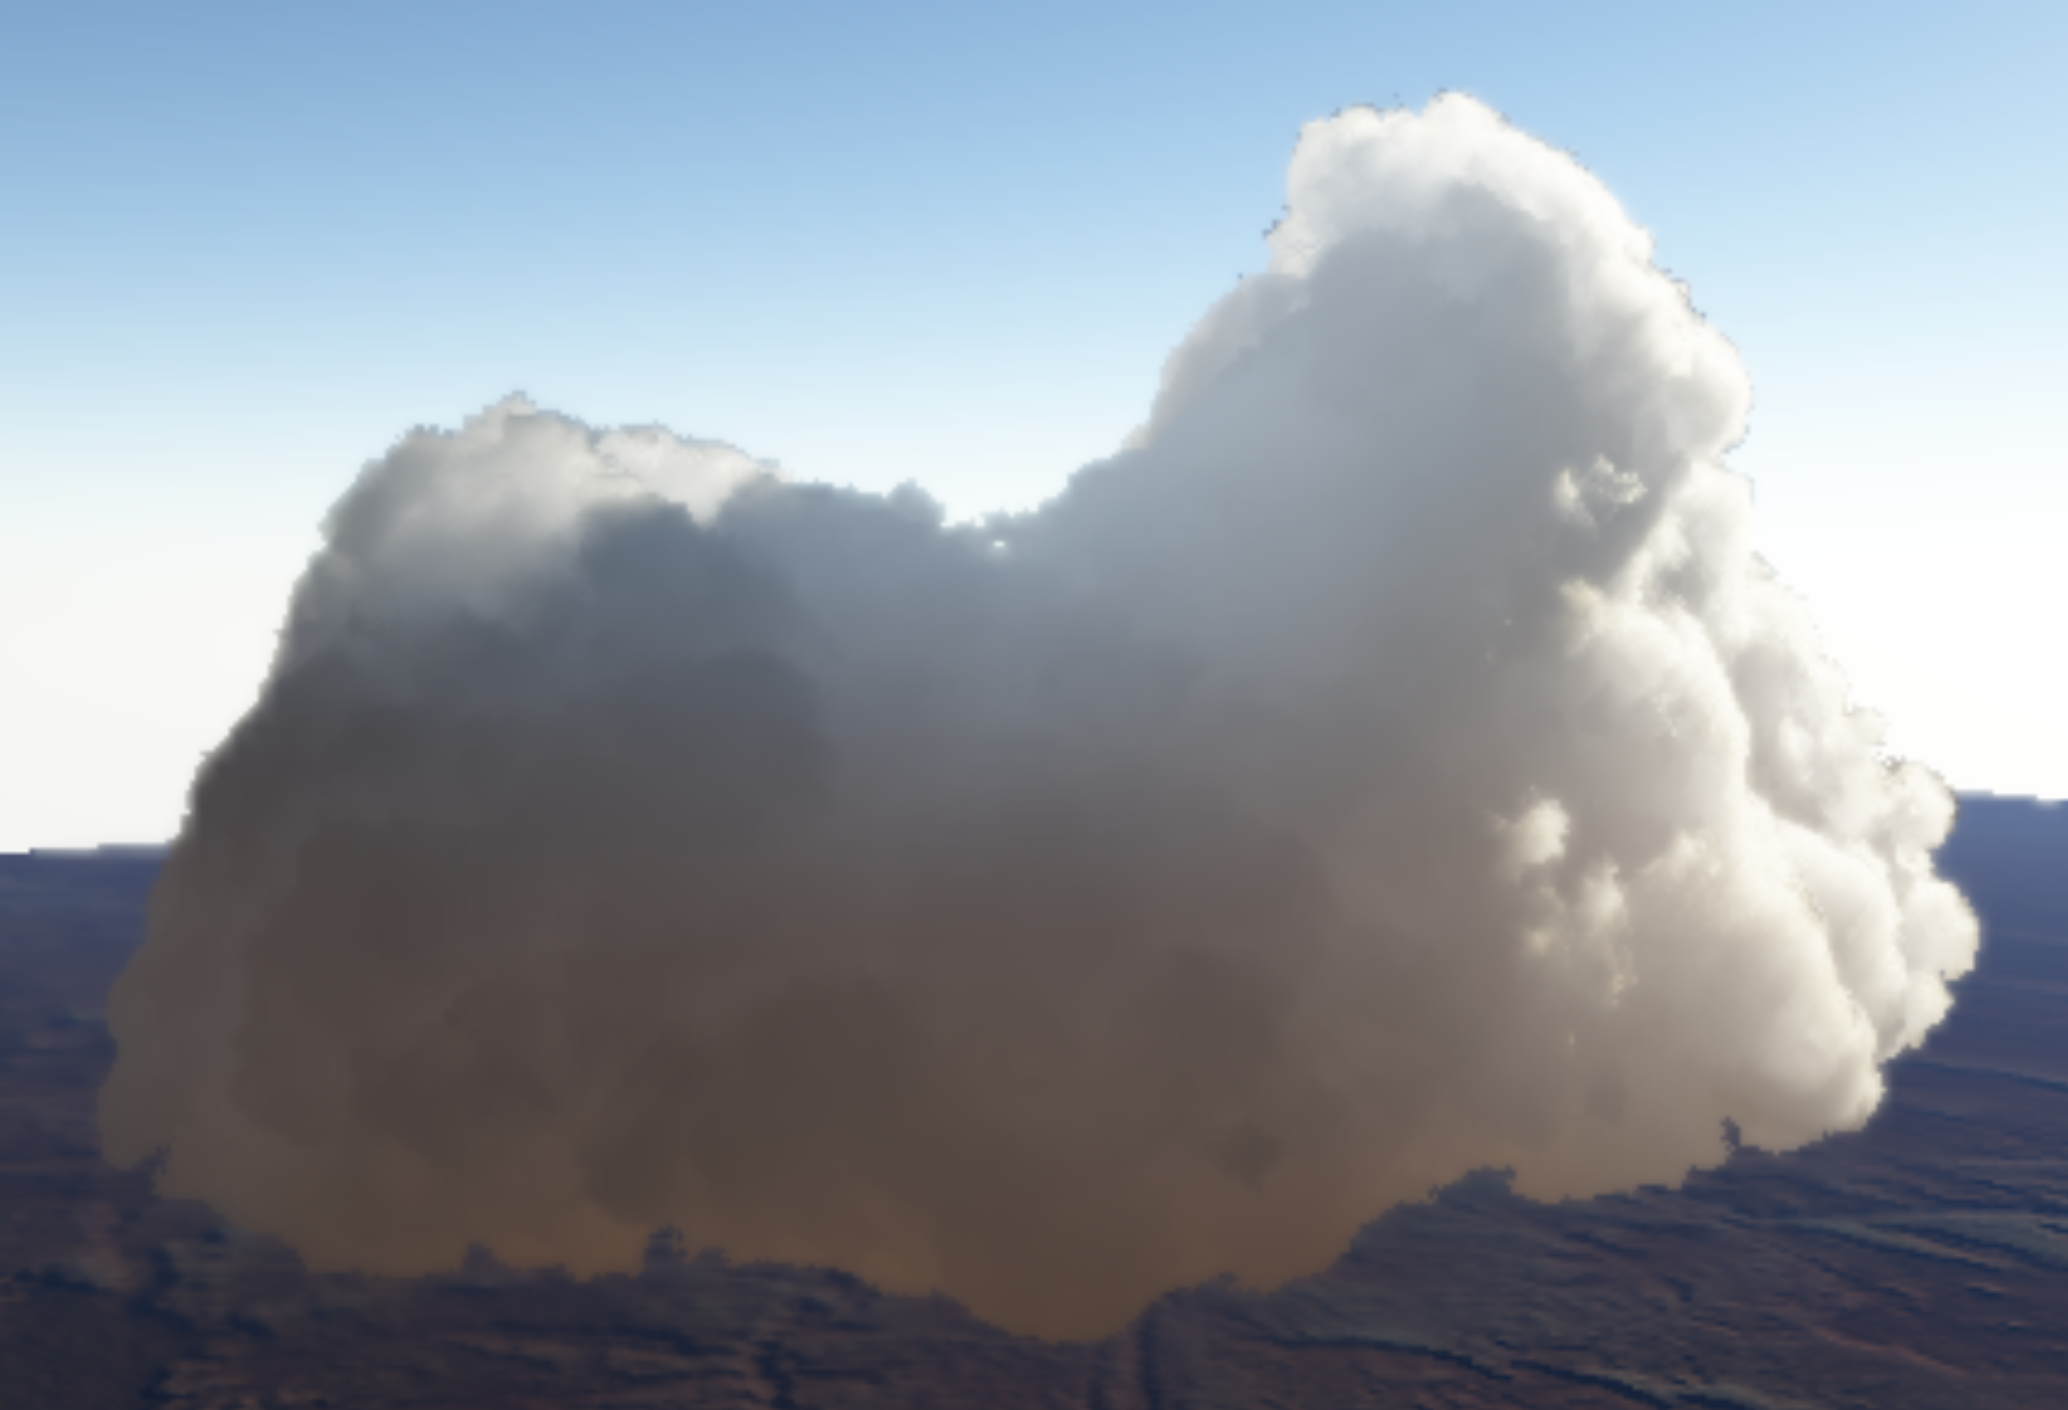
\includegraphics[scale=0.4]{img/raymach.png}
    \caption{Результат алгоритма лучевого марша}
    \label{img:raymach}
\end{figure}

Из таблицы \ref{table:clouds} видно, что алгоритм, использующий текстуру не подходит, поскольку необходимо генерировать
объемные облака с динамическим освещением. Трассировка лучей не подходит из-за высокой трудоемкости. Исходя из этого,
можно сделать вывод, что выгоднее всего использовать алгоритм, использующий частицы.

\begin{table}[H]
    \centering
    \caption{Сравнение алгоритмов генерации облаков}
    \label{table:clouds}
    \begin{tabular}{|c||c|c|}
        \hline
        Алгоритм & Динамическое освещение и объем & Скорость \\
        \hline
        \hline
        Текстура на сфере & -- & + \\
        \hline
        Частицы & + & + \\
        \hline
        Трассировка лучей & + & -- \\
        \hline
    \end{tabular}
\end{table}

\section{Градиентные шумы}

Для генерации форм и текстур облаков используются алгоритмы градиентных шумов.
Шум это беспорядочные колебания физической природы. В данной работе используется два алгоритма
генерации шумов: Перлина и Уорли.

\subsection{Шум Перлина}

Шум перлина применяется для любого $n$-мерного пространства. Данный алгоритм состоит из трех этапов.

Пространство делится $n$-мерной сеткой, которая заполняется псевдослучайными единичными векторами \cite{Perlin}.
На рисунке \ref{img:vectors} представлен пример для 2-мерного пространства.

\begin{figure}[H]
    \centering
    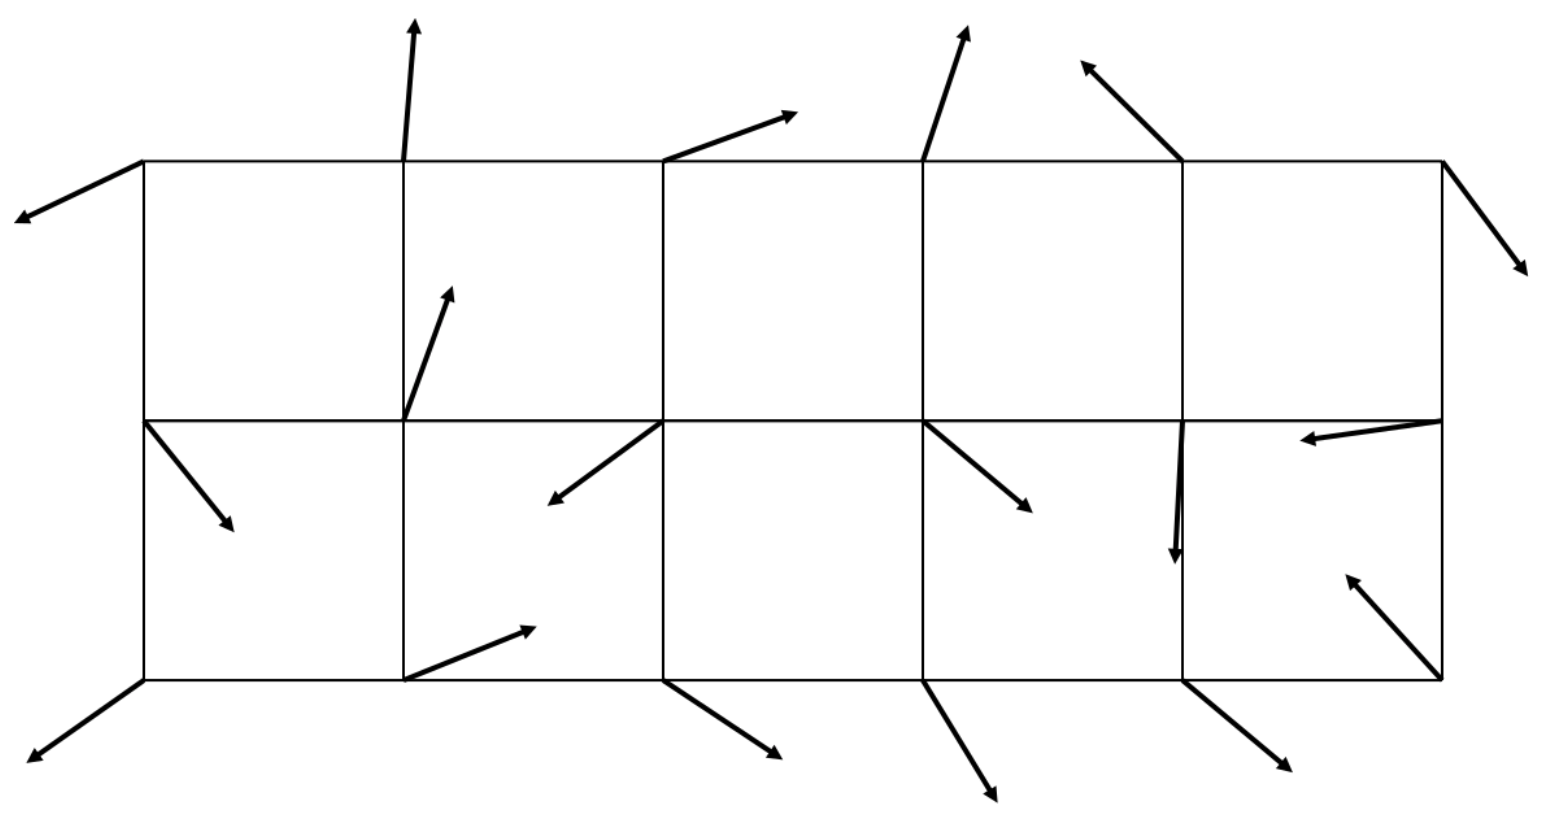
\includegraphics[scale=0.6]{img/vectors.png}
    \caption{Сетка псевдослучайных векторов}
    \label{img:vectors}
\end{figure}

После необходимо интерполировать значения внутри сетки. Делается это при помощи скалярного произведения векторов \ref{eq:scalar}.
Каждая точка сетки имеет два вектора: ранее сгенерированный и указывающий на текущую точку \cite{Perlin} (рисунок \ref{img:interpolation}).

\begin{equation}\label{eq:scalar}
    \vec a \cdot \vec b = a_x \cdot b_x + a_y \cdot b_y
\end{equation}

\begin{figure}[H]
    \centering
    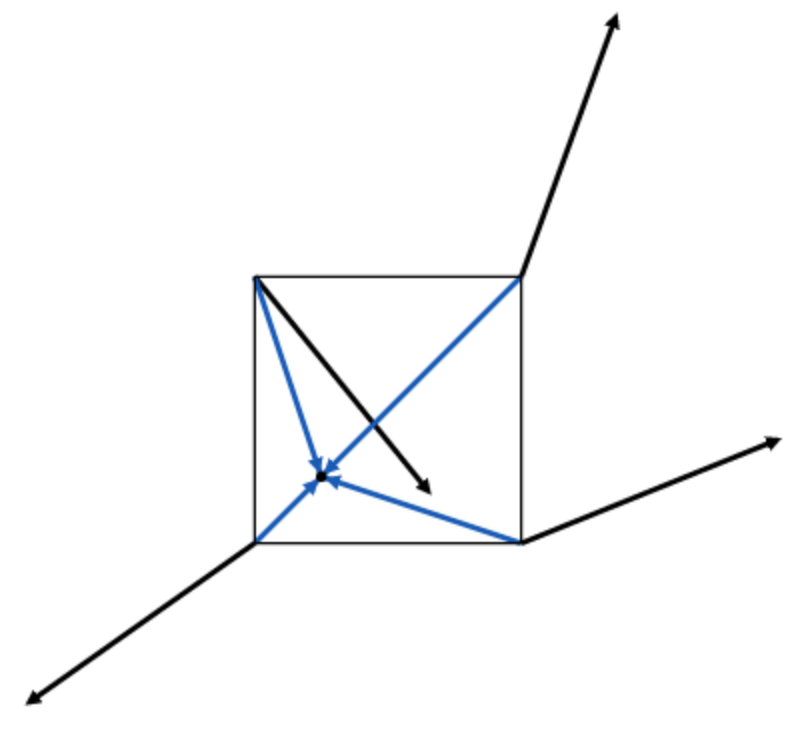
\includegraphics[scale=0.6]{img/interpolation.png}
    \caption{Интерполяция значений шума}
    \label{img:interpolation}
\end{figure}

Для каждой точки пространства есть четыре скалярных произведения, поскольку имеется 4 соседние вершины сетки.
Для скалярных произведений дважды применяется интерполяция для двух значений \ref{eq:interpolation}.
И полученные два значения также интерполируются \cite{Perlin}. После проделанных операций получается слишком
гладкий шум. Для увеличния эффекта облачности необходимо взять такой же результат, с увеличенным в два раза разрешением,
разделить выходные значения на $2$ и прибавить к исходному графику. Это называется октавами, которые можно проделать сколько угодно
раз. После 8 октав получается шум, указанный на рисунке \ref{img:perlin}.

\begin{equation}\label{eq:interpolation}
    f(t) = a_1 \cdot t + a_0 \cdot (1 - t), 0 \le t \le 1
\end{equation}

\begin{figure}[H]
    \centering
    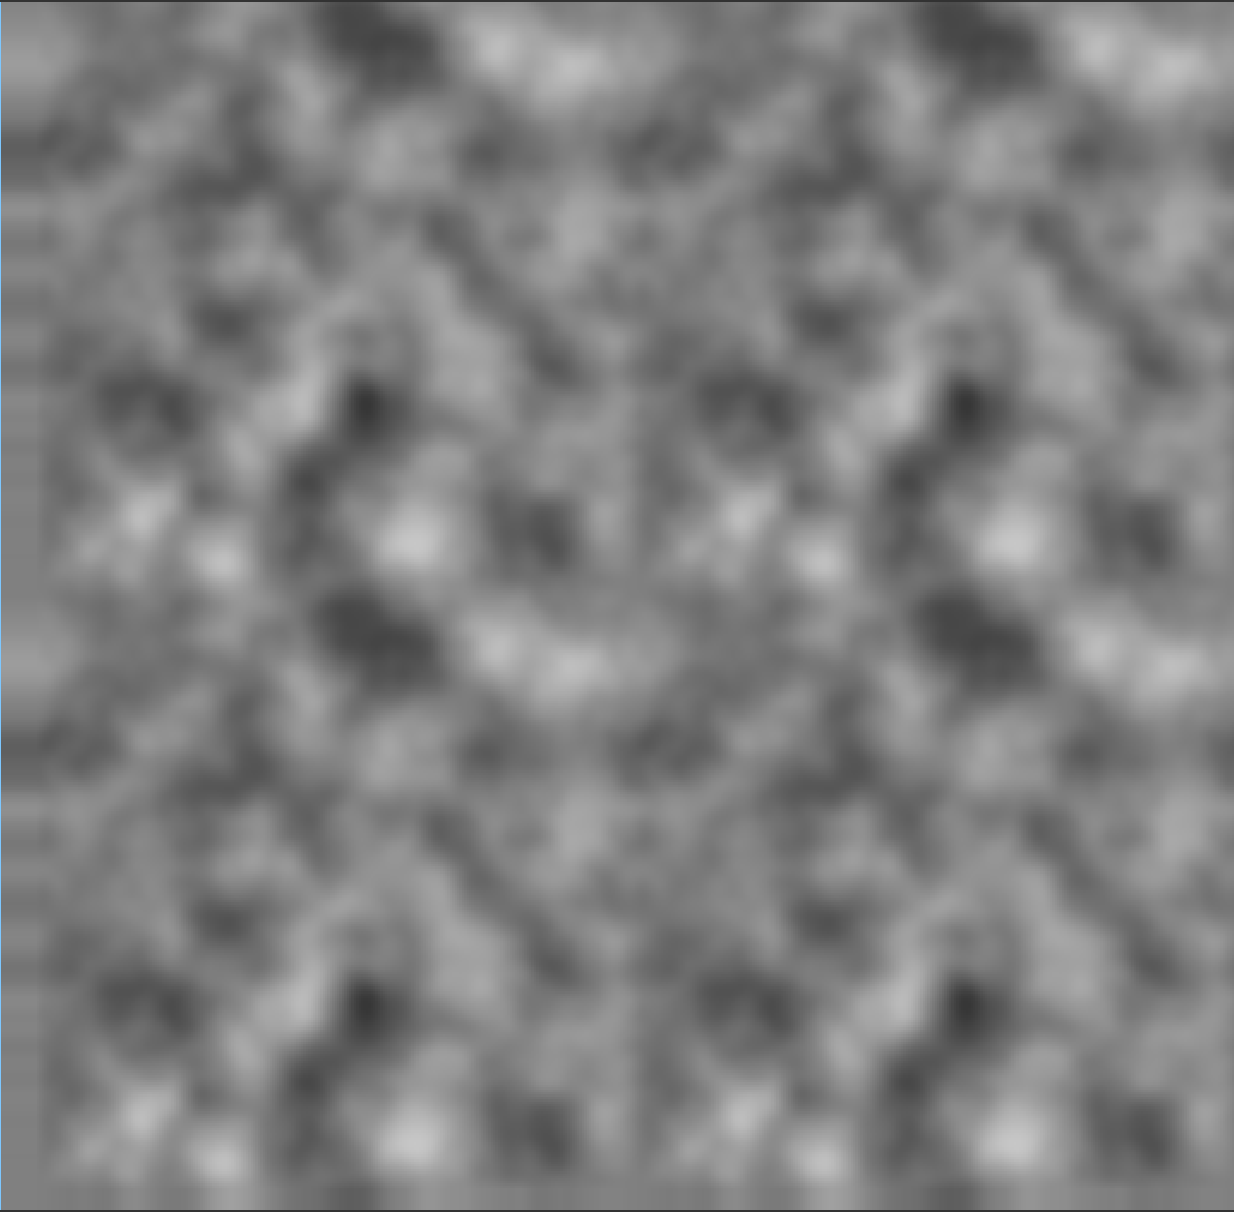
\includegraphics[scale=0.4]{img/perlin.png}
    \caption{Шум Перлина}
    \label{img:perlin}
\end{figure}

\subsection{Шум Уорли}

Основная идея шума Уорли состоит в том, чтобы случайным образом или используя закон распределения
расбросать точки в $n$-мерном пространстве. Затем для каждой координаты находятся расстояния до
ближайших точек, которые сортируются по возрастанию расстояний. Для итогового результата берется расстояние
до $N$-й точки (обычно $N=2$ или $N=4$) среди отсортированных расстояний \cite{Worley}.
Результат видно на рисунке \ref{img:worley}

\begin{figure}[H]
    \centering
    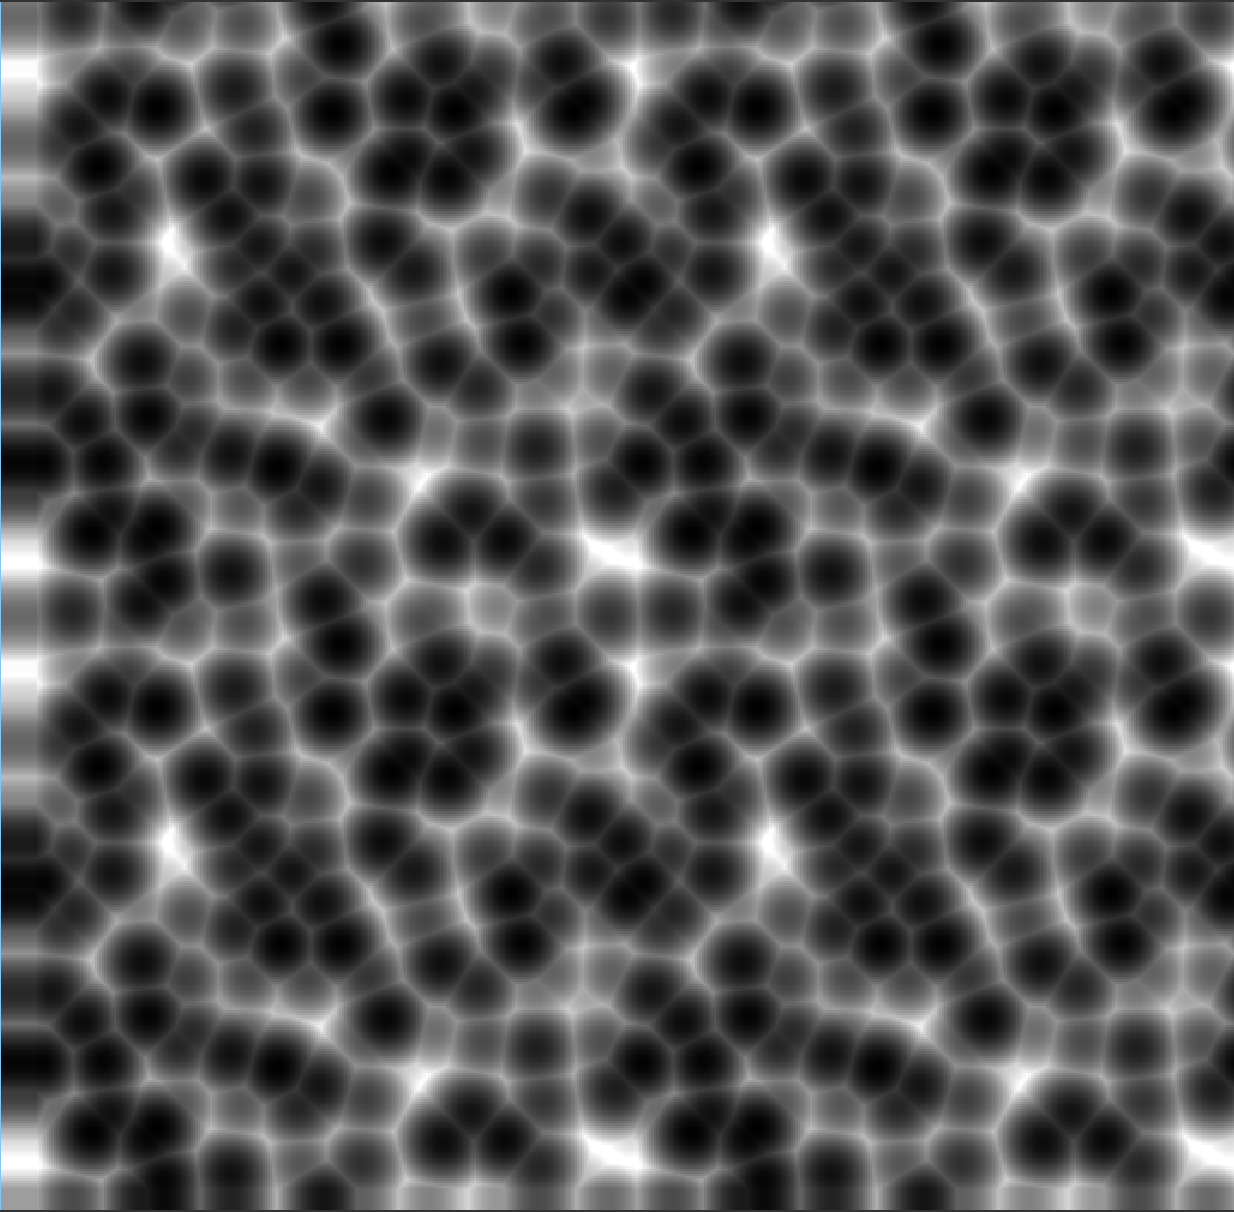
\includegraphics[scale=0.4]{img/worley.png}
    \caption{Шум Уорли}
    \label{img:worley}
\end{figure}

\section{Тени}

Реалистичное изображение не может быть без теней. Для реализации теней используется алгоритм, использующий
буфер глубины. При испоьзовании данного алгоритма сцена отрисовывается со взгляда источника света, а для каждой
точки сохраняется значение ближайшей к источнику, чтобы в будущем затенить остальные, которые являются невидимыми
для источника света.

Во время отрисовки сцены необходимо совместить каждую точку с точкой на буфере глубины и сравнить значение глубины.
Для совмещения используются преобразования к виду от лица источника света, как было при первой этапе.
Если глубина оказалась меньше, то точку необходимо затенить \cite{shadowmapping}.

При заполнении карты используются ортогональные тени, то есть источником света является Солнце, все лучи которого
параллельны (рисунок \ref{img:shadow}).

\begin{figure}[H]
    \centering
    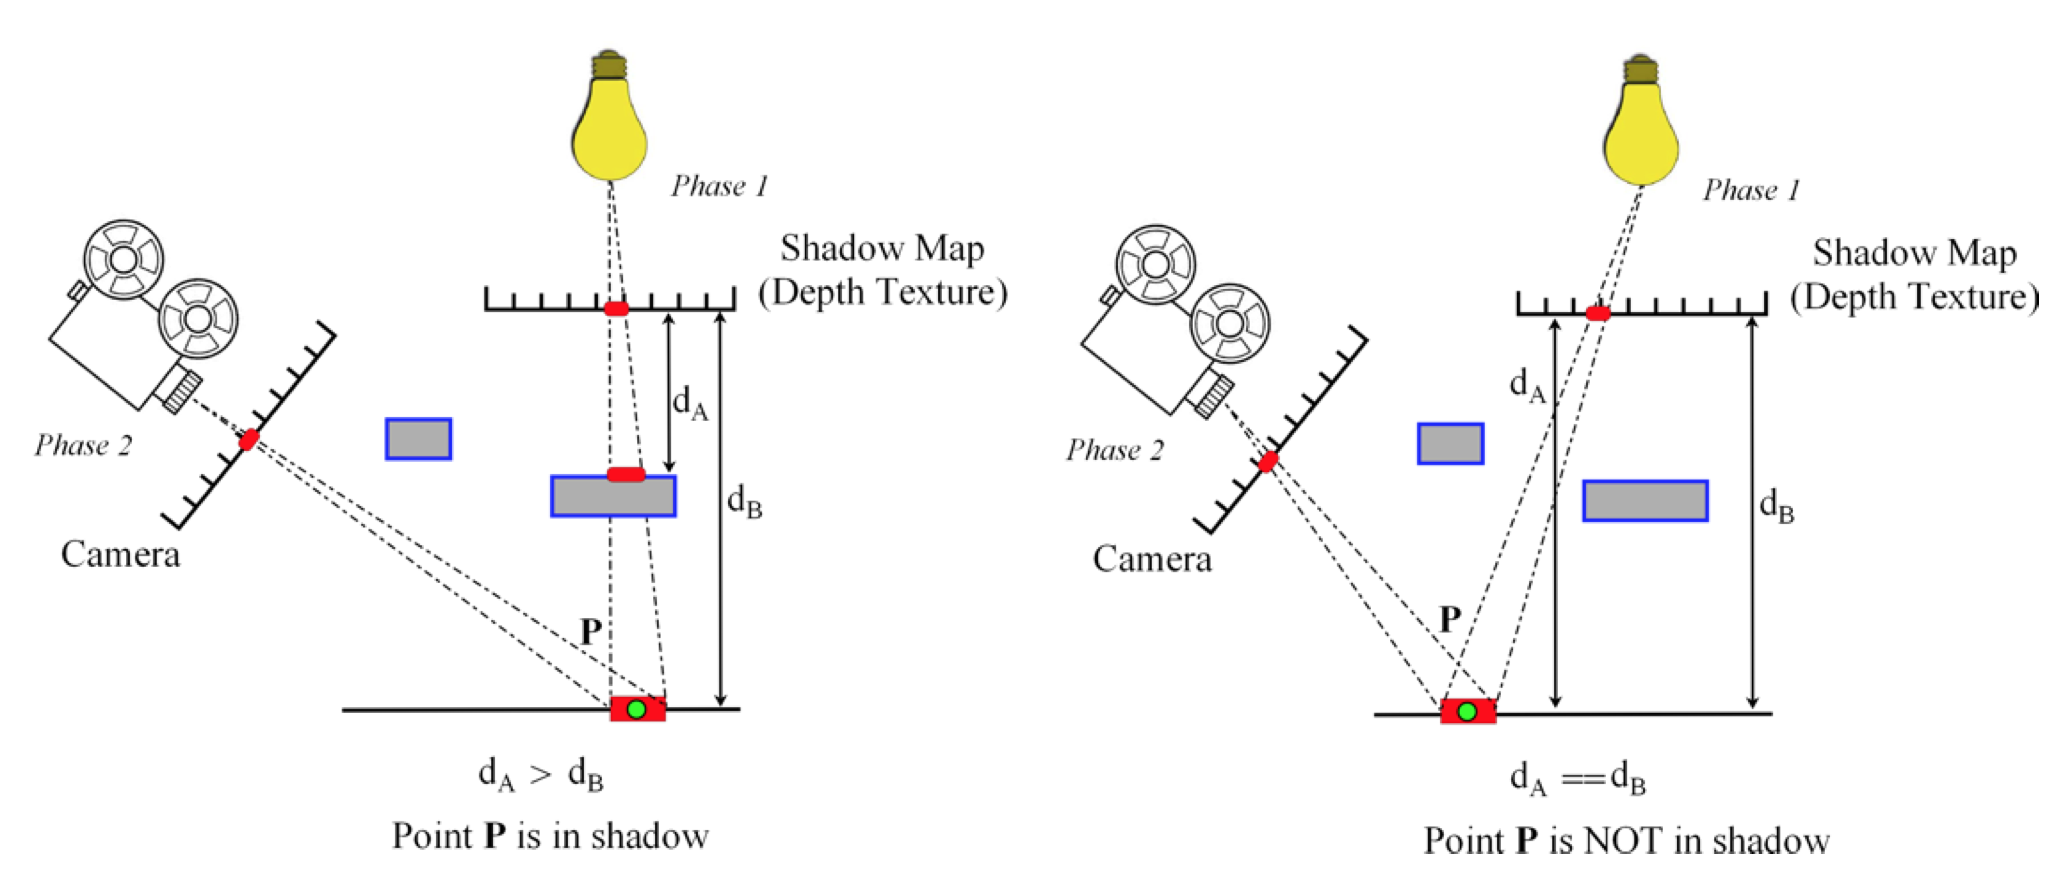
\includegraphics[scale=0.4]{img/shadow.png}
    \caption{Метод теневых карт для ортогональных теней}
    \label{img:shadow}
\end{figure}

\section{Выводы}

Таким образом, используя выбранные алгоритмы можно сгенерировать и визуализаровать объемные облака,
рендеринг которых востребован для таких целей, как авиасимуляторы или видеоигры, где необходимо
создавать ощущение настоящих облаков.
